% !TEX program = xelatex
\documentclass{article}
\usepackage{xeCJK}
\setCJKmainfont[
    BoldFont=cwTeXQHei-Bold,
    ItalicFont=cwTeXQYuan-Medium,
    Scale=1.1
]{cwTeXQFangsong-Medium}
\usepackage{/Users/jay/LaTeX/cs}
\usepackage{/Users/jay/LaTeX/codelist}

\newcommand{\hmwkClass}{Operating System, Spring 2018}
\newcommand{\hmwkTitle}{Project 1}
\newcommand{\hmwkDueDate}{April 14, 2018}
\newcommand{\tb}{\textbf}

\begin{document}

\thispagestyle{empty}
\section*{\hmwkClass \\
    \normalsize{\hmwkTitle} \\
    \normalsize{DUE DATE: \hmwkDueDate}
}

\hfill{Team 16: \, B03505053 \, 曾彥青 \, B03902129 \, 陳鵬宇} \\

\subsection*{Implementation details or faced difficulties}

To implement this project, we simply followed the specs in the pdf. The first difficult we faced is that when typing

\begin{lstlisting}
  $ sudo make menuconfig
\end{lstlisting}

it came up with the following error messages:

\begin{figure}[!htb]
    \centering
    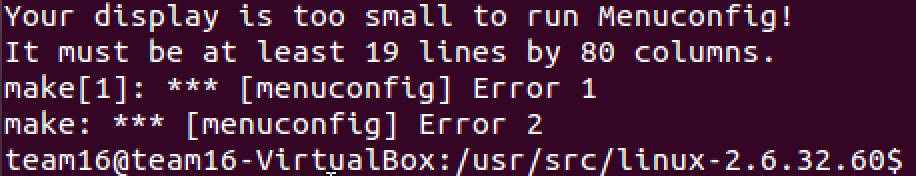
\includegraphics[width=0.5\textwidth]{img/Menuconfig.png}
    \caption{Menuconfig Error}
\end{figure}

We solved it by typing:

\begin{lstlisting}
    sudo apt-get install virtualbox-guest-dkms virtualbox-guest-utils virtualbox-guest-x11
\end{lstlisting}

in the \tb{Terminal}. \\

In \tb{"/usr/src/linux-2.6.32.60/arch/x86/kernel/syscall\_table\_32.S"}, we added

\begin{figure}[!htb]
    \centering
    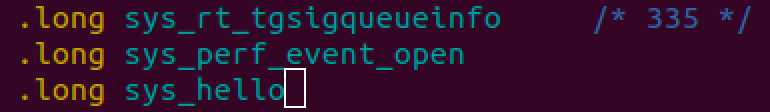
\includegraphics[width=0.5\textwidth]{img/syscall_table.png}
    \caption{syscall\_table\_32.S}
\end{figure}

In \tb{"/usr/src/linux-2.6.32.60/arch/x86/include/asm/unistd\_32.h"}, we added

\begin{figure}[!htb]
    \centering
    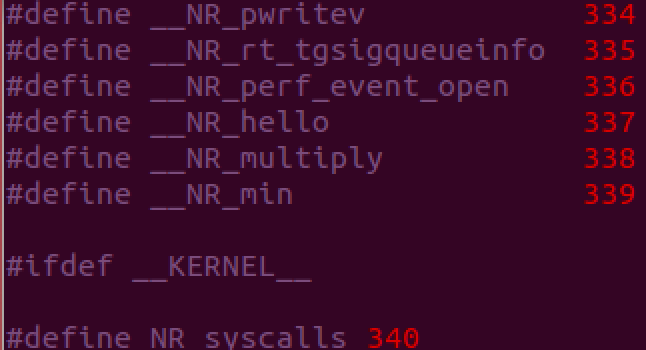
\includegraphics[width=0.5\textwidth]{img/unistd_32.png}
    \caption{unistd\_32.h}
\end{figure}

\newpage
In \tb{"/usr/src/linux-2.6.32.60/arch/x86/include/asm/syscalls.h"}, we added

\begin{figure}[!htb]
    \centering
    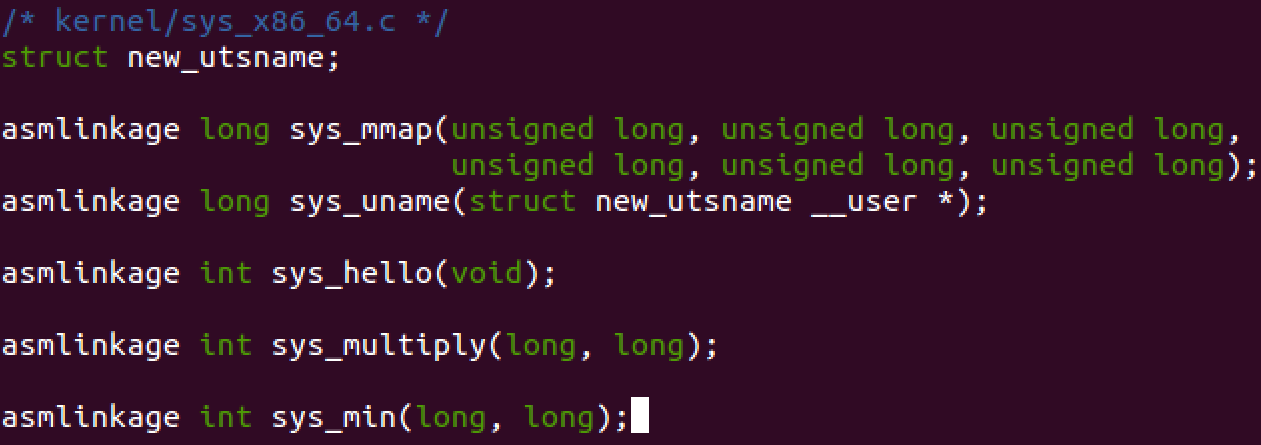
\includegraphics[width=0.5\textwidth]{img/syscalls.png}
    \caption{syscalls.h}
\end{figure}

\subsection*{Our results}

Our test program:

\begin{figure}[!htb]
    \centering
    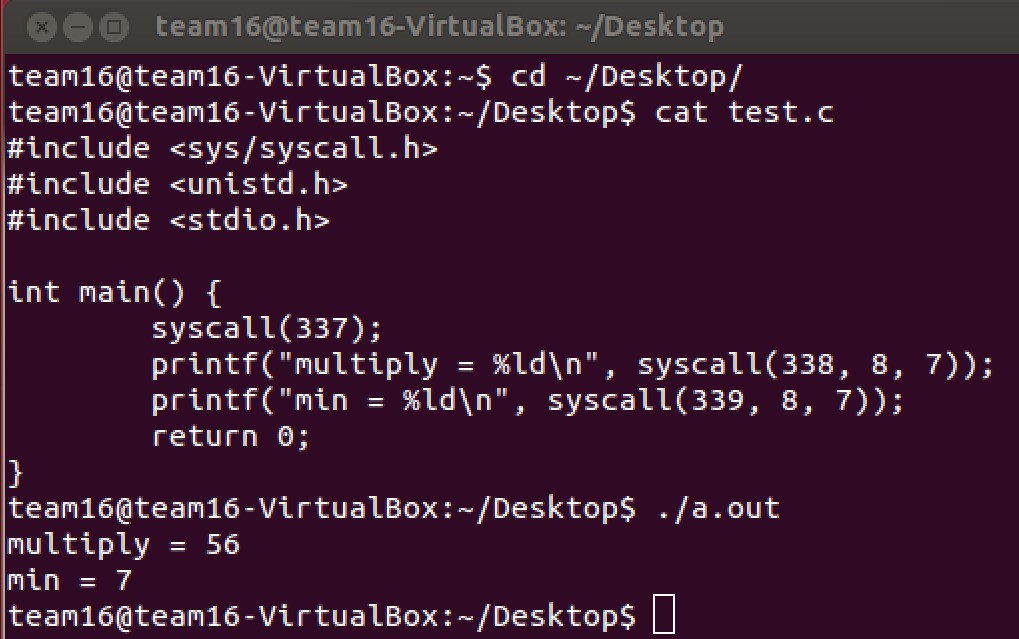
\includegraphics[width=0.5\textwidth]{img/test.png}
    \caption{test.c}
\end{figure}

After typing \tb{"dmesg"},

\begin{figure}[!htb]
    \centering
    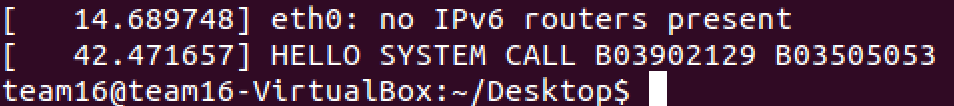
\includegraphics[width=0.5\textwidth]{img/studentID.png}
    \caption{dmesg}
\end{figure}

it correctly showed up our student IDs.

\end{document}